 %!TEX root = ../dokumentation.tex

%TODO: Einleitungen überarbeiten
\chapter{Concept}\label{cha:Concept}
This chapter outlines the concept and the architecture of the software tool.
First, in section \ref{sec:ConceptRequirements}, the requirements the software tool needs to meet are described.
Then, in section \ref{sec:ConceptOverview}, the components needed are introduced.
 Then the proposed software architecture is described. After that the concept of each component is developed.

why python

\section{Requirements}\label{sec:ConceptRequirements}
The tool should meet the following requirements:\\
The tool has a GUI that is the interface between the tool and a user. Hence, the user communicates with the tool via the GUI. The user should be able to import a grammar file. After the grammar file is imported, the grammar file should be displayed. 
This includes displaying by the grammar defined productions as well as comments that are associated with grammar productions.
The user can select a new start symbol and can select which productions should be blocked. 
Productions can either be blocked as a whole or partly if the production is a disjunction.
After the user made his choice, the new reduced grammar should be generated and displayed.
The tool should also generate a control file listing blocked productions and the start symbol.
Furthermore, the tool should be able to import a control file and reduce a given grammar based on this control file instead of reducing a grammar based on a users selection of blocked productions.
The new reduced grammar should be exported to .txt format.
Also, comments referring to the remaining productions should be kept and comments referring to productions that fell away should not be included in the new grammar.

\section{Overview}\label{sec:ConceptOverview}

Figure \ref{fig:ConceptProcessSublanguage} outlines the procedure of extracting a sublanguage of the \ac{TPTP} language.
The first task is to import the \ac{TPTP} language grammar specification file and extract the tokens using the lexer.
The next phase is for the parser to create a data structure from the tokens, also checking if the syntax in the grammar file was correct.
Then, a graph representing the imported \ac{TPTP} grammar should be built.\\
This graph is subject to manipulation by disabling certain transitions or selecting a new start symbol in the following phase.
This includes computation of the remaining reachable and terminating grammar.
That new graph represents the grammar of the extracted language.
To make this grammar usable, lastly the language specification has to printed, based on the new graph, in the same format as the original language specification.
\begin{figure}[H]
\tikzstyle{decision} = [ diamond, draw, fill=blue!10, text width=4.5em, text badly centered, node distance=2cm, inner sep-0pt]  
\tikzstyle{block} = [ rectangle, draw, fill=blue!10, text width=4.5em, text badly centered, rounded corners, minimum height=4em]  
\tikzstyle{line} = [ draw, -latex']  
%\tikzstyle{terminator} = [ draw, ellipse, fill=red!20, node distance=3cm, minimum height=2em]
\tikzstyle{terminator} = [rectangle, draw, fill=blue!10, text width=4.5em, text badly centered, rounded corners, minimum height=4em]  
\begin{center}
\begin{tikzpicture}[node distance=3cm, auto]  
  %\node [terminator]           (import)  {Import grammar file};  
  %\node [terminator]           (import)  {Import of grammar file};
  \node [terminator]  (lex)  {Import of grammar file and lexing};  
  \node [block, right of=lex]  (pars) {Parsing};  
  \node [block, right of=pars] (ggg) {Grammar graph generation}; 
  \node [block, right of=ggg] (ggm) {Grammar graph modification}; 
    \node [block, right of=ggm] (go) {Grammar output};  
  %\path [line] (import)  -- (lex);  
  \path [line] (lex)  -- (pars);  
  \path [line] (pars) -- (ggg);  
  \path [line] (ggg) -- (ggm); 
  \path [line] (ggm) -- (go);  
\end{tikzpicture}
\end{center}
\caption{Procedure of extracting a sublanguage}
\label{fig:ConceptProcessSublanguage}
\end{figure}

\subsection{Proposed Architecture}\label{sec:ConceptProposedArchitecture}
The architecture of the software tool should take the procedure of extracting a sublanguage (section \ref{sec:ConceptOverview}) into consideration.
From that, five main components can be identified:
An import module responsible for importing the \ac{TPTP} language specification from a file;
A lexer for extracting tokens from the language specification; A parser for creating a data structure from the tokens;
A graph builder and manipulator;
An export module for exporting the graph in a text representation corresponding to the original language specification.\\
In addition to the components that provide the main functionality a graphical user interface and a console interface for user convenience is desired.

todo architecture diagram

\section{Lexer}\label{sec:ConceptLexer}
The lexer is responsible for extracting the tokens from the \ac{TPTP} language grammar specification file.
todo why lexer with ply, what does ply help
\ac{PLY} offers a lexer generator for python (see section \ref{sec:BackgroundPLY}).
Using \ac{PLY} a lexer can be built by specifying tokens as regular expressions.

Therefore the \ac{TPTP} language grammar specification needs to be analysed in order to find elementary tokens and regular expressions, that precisely describe these tokens.
\subsection{Elementary Tokens}\label{sec:ConceptElementaryTokens}
todo check if bnf or ebnf

The grammar of the \ac{TPTP} language is specified in a modified \ac{EBNF} todo source.
Therefore there are deviations from standard \ac{EBNF} (see \ref{sec:BackgroundBNF}) that need to be analysed to specify elementary tokens.
The standard \ac{EBNF} only uses one production symbol ($"::="$).
In the \ac{TPTP} language additional production symbols have been added.
The following table \ref{tbl:ConceptTPTPProductionSymbols} contains the production symbols used in the \ac{TPTP} language, that also have to be recognized by the lexer.
\begin{table}[H]
\centering
\renewcommand{\arraystretch}{1}
\caption{\ac{TPTP} language production symbols \cite{VS06}}
\begin{tabular}{ll}
\textbf{Symbol} & \textbf{Rule Type}\\\hline
::= & Grammar\\
:== & Strict\\
::- & Token\\
::: & Macro\\
\end{tabular}
\label{tbl:ConceptTPTPProductionSymbols}
\end{table}

Another deviation from \ac{EBNF} is that repetition is not denoted by surrounding curly brackets, but with a trailing $*$ symbol.\\
Curly brackets have no special meaning in the \ac{TPTP} laguage grammar specification and can be treated as terminal symbols.\\
The meaning of the alternative symbol $|$ is unchanged and also parentheses and square brackets can appear as meta symbols.\\
Also, there are line comments in the \ac{TPTP} language specification.
A comment starts with the $\%$ symbol at the beginning of a line and ends at the end of that line.\\
Following standard \ac {BNF}, nonterminal symbols are enclosed by the $<$ and $>$ symbol and terminal symbols are written without any special marking.

todo regular expressions
 
todo explain token nt symbol + production rule bc. of parser
\subsection{Regular Expressions}\label{sec:ConceptRegularExpressions}

\section{Parser}\label{ConceptParser}
The goal that the parser component should fulfil is to take the tokens from the lexer as input and create a data structure that represents the structure of the \ac{TPTP} language grammar specification sign.
To create the parser the \ac{PLY} parser generator is used.

-rules have to be defined

In the \ac{TPTP} language specification square brackets not necessarily denote that an expression is optional.
In token and macro rules they have the same meaning as in traditional \ac{EBNF} and in grammar and semantic rules square brackets are terminals.

\subsection{Data Structure and Data Types}\label{sec:ConceptParserDataStructure}
To build the representative data structure, data types that represent the data stored in the \ac{TPTP} language grammar specification have to be defined.
The following section describes the data structure and data types that are being used and created by the parser in the parsing process.

Atomary data types

\subsubsection{Terminal Symbol}
The terminal symbol data type has one attribute, which is the name of the terminal symbol.
-todo Production Property

\subsubsection{Nonterminal Symbol}
Analogue to the terminal symbol data type, the nonterminal symbol also has its name as an attribute.

Composite data types

\subsubsection{Expressions}
%\subsubsection{Grammar Expression}
An expression consists of the nonterminal symbol name which is produced, a production list and a position.
The position denotes at which position in the \ac{TPTP} language grammar specification the grammar expression was listed.
This information is needed to maintain the original order of the expressions when printing the reduced grammar specification (todo reference).\\
For each production symbol (see table \ref{tbl:ConceptTPTPProductionSymbols}) there is a data type. This means that grammar, token, strict and macro expression data types are introduced.\\
Listing \ref{lst:ConceptParserGrammarExpression} contains an example of a line in a \ac{TPTP} language grammar specification that is represented by the grammar expression data type.
\begin{lstlisting}[basicstyle=\scriptsize	,caption= Example of a grammar expression,label= lst:ConceptParserGrammarExpression]
<tff_formula>          ::= <tff_logic_formula> | <tff_atom_typing
\end{lstlisting}
The nonterminal symbol name which is produced is <$tff \textunderscore formula$>.  The production list consists of two productions, as can be seen in the listing.
\subsubsection{Comment Block}
A comment block is a list of consecutive comment lines.

\subsubsection{Production Element}
A production element is.
-terminal symbol
-nonterminal symbol
-production property
\subsubsection{Production Property}
The production property can take one of three values and denotes whether a production is optional, can be repeated any number of times or does not have any special property. In the original \ac{TPTP} language grammar specification file this was represented by square brackets or the repetition symbol.


\subsubsection{Production}
A production is one production alternative specified in any expression. It consists of a list of production elements and has a production property.
-show example
\subsubsection{Production Property}
-none
-repetition
-optional
\subsubsection{Productions List}
A productions list contains a list of productions where each production is one alternative in the description of an expression.
\subsubsection{XOR Productions List}
Multiple alternatives enclosed by parantheses.

\subsubsection{Grammar List}
The grammar list is the top level data structure. It contains a list of all elements that were in the \ac{TPTP} language specification file. This includes any type of expression (grammar, token, strict and macro) and comment blocks.

\subsection{Production Rules}


The output of the parser is a list of the rules and the comments from the \ac{TPTP} language specification file.
\section{Graph Generation}\label{sec:ConceptGraphGeneration}
The \ac{TPTP} grammar, extracted from the \ac{TPTP} grammar file, needs to be stored in a data structure that allows for modification.
A graph representing possible transitions within the 
-number rules
-challenge that one start symbol can have multiple rule types
-uml NTNode

\begin{figure}
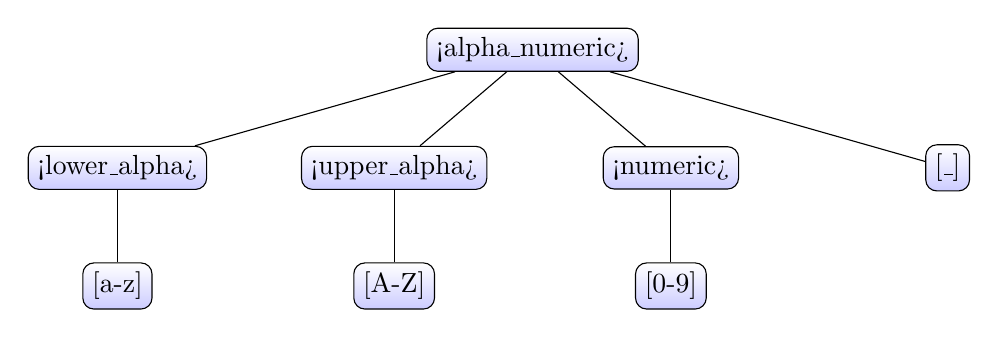
\begin{tikzpicture}[sibling distance=10em,
  every node/.style = {shape=rectangle, rounded corners,
    draw, align=center,
    top color=white, bottom color=blue!20}]]
  \node {<alpha\textunderscore numeric>}
    child { node {<lower\textunderscore alpha>} 
    	child { node {[a-z]}}}
    child { node {<upper\textunderscore alpha>}
      child { node {[A-Z]}}}
    child { node {<numeric>}
    	child { node {[0-9]}}}
    child { node {[\textunderscore]}};
\end{tikzpicture}
\caption{Example of parse tree}
\end{figure}

Circular dependency:
\begin{lstlisting}[basicstyle=\scriptsize	,caption= Example of a circular dependency,label= lst:GraphGeneration_circular_dependency]
<disjunction>    ::= <literal> | <disjunction> <vline> <literal>
\end{lstlisting}

The graph is generated recursive. 
Idea:  

\section{Generation of the reduced Grammar}\label{sec:ConceptGenerateReducedGrammar}

\subsection{Selection of blocked Productions}

\subsection{Determination of the remaining reachable Productions}

\subsection{Determination of the remaining terminating Productions}

\section{Control File}\label{sec:ConceptControlFile}
A format for specifying the desired start symbol and blocked productions has to be developed.
Using a file-based configuration enables the user to store desired configurations and for example a manual selection in the graphical user interface is not necessary.
It also helps with using the command line interface, because there manual selection is not possible.
The file should be human-readable and -editable.\\
The format should be easy to parse and allow to specify all necessary information.
This includes the desired start symbol and all production rules that should be blocked.\\
The proposed way to describe this information is to:

\begin{itemize}%[noitemsep]
	\item define the desired start symbol in the first line.
	\item define blocked productions grouped by nonterminal symbol and production symbol separating each group by a new line.
	First defining the nonterminal symbol, then the production symbol and after that the index of the alternatives that should be blocked (indexing starts at zero). 
\end{itemize}
\label{itemize:ConceptControlFile}
Identifying the production symbol is necessary because there may be a nonterminal symbol that has productions with more than one production symbol.\\
Listing \ref{lst:ConceptControlFile} contains a sample control file. In this file in the first line <$TPTP\_File$> is specified as start symbol.
The second line means, that the second grammar production alternative of the nonterminal symbol <$TPTP\_input$> should be disabled.
Analogue to that, the first, second, third and fifth grammar production alternative of the nonterminal symbol <$annotated\_formula$> are said to be disabled in line 3.

todo further describe control file, is it understood, which production is disabled? maybe graphical help??
\begin{lstlisting}[caption= Example of a control file,label= lst:ConceptControlFile]
<TPTP_file>
<TPTP_input>,::=,1
<annotated_formula>,::=,0,1,2,5
\end{lstlisting}
This format is relatively easy to parse and also enables users to specify their desired start symbols and blocked productions without having to use the GUI.

pro: Specifying which production should be blocked, and not the ones should be kept, typically results in a significantly smaller file.
Storing the indexes of the productions that should be blocked offers that in case productions are renamed the control file would still be valid. On the other hand if productions are added or deleted from the original \ac{TPTP} language grammar specification, the control file may have to be updated.


\section{Maintainig Comments}\label{sec:ConceptMaintainingComments}
In the \ac{TPTP} language specification there are comments providing supplemental information about the language and its symbols and rules.
When generating a reduced grammar maintaining of comments is desired. This means that comments from the original language specification should be associated with the rule they belong to and if the rule is still present in the reduced grammar, also the comment should be.\\
Therefore a mechanism has to be designed for the association of comments to grammar rules.

Listing \ref{lst:ConceptComment_tptp} features an example of a comment in the \ac{TPTP} laguage specification.
\begin{lstlisting}[basicstyle=\scriptsize	,caption= Example of a comment in the \ac{TPTP} language specification,label= lst:ConceptComment_tptp]
%----Top of Page---------------------------------------------------------------
%----TFF formulae.
<tff_formula>          ::= <tff_logic_formula> | <tff_atom_typing> |
                           			  <tff_subtype> | <tfx_sequent>
\end{lstlisting}
heuristic:
comments near the rule the refer to
associate comment with r

bei tree building temporäres startsymbol nutzen (da mehrere Startsymbole möglich)

\begin{figure}[H]
\centering
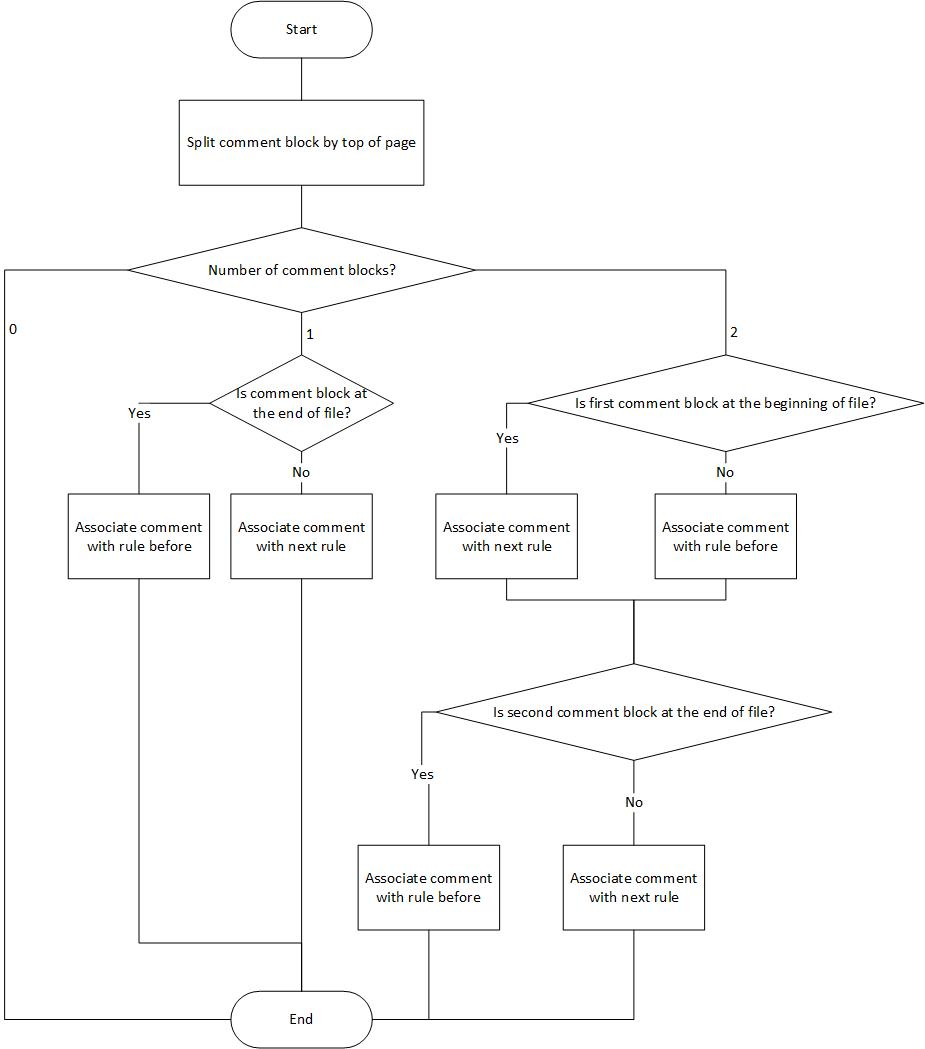
\includegraphics[width=1\textwidth]{images/maintainingComments.jpg}
\caption{Maintaining Comments}
\label{fig:comments}
\end{figure}

\section{Console Interface}\label{sec:Console Interface}
-output reduced grammar with input grammar control file 
\section{GUI}\label{sec:ConceptGUI}
-show rules similar to file
-select start symbol + blocked productions
-show extracted grammar
-export exported grammar
-include + toggle comments
-import/export control file
extra:
-web import


